So far, we have learnt two equivalent descriptions of the concept of continuity for functions $f: (X,d) \to (Y, \overset{\sim}{d}):$
(1) $f$ is continuous if and only if
$$\forall c \in X ~\forall \epsilon > 0 ~\exists \delta_{\epsilon, c} > 0 \st \text{if $d(x,c) < \delta_{\epsilon, c}$ then $\overset{\sim}{d}(f(x), f(c)) < \epsilon$}$$
(2) $f$ is continuous if and only if
$$\forall c \in X ~a_n \to c \implies f(a_n) \to f(c).$$
Our next goal is to describe a third (equivalent) description of continuity. \\ \\
In Math 130: $f:\R \to \R, a_n \to c$ in $\R$
$$a_n \to c \iff \forall \epsilon > 0 ~\exists N \st \forall n > N ~~|a_n - c| < \epsilon.$$
Math 230: $(X,d)$
\begin{align*}
    &\text{Level 1:} && a_n \to c \iff \forall \epsilon > 0 ~\exists N \st \forall n > N ~~d(a_n, c) < \epsilon \\
    &\text{Level 2:} && a_n \to c \iff \forall \nbhd{\epsilon}{c} ~\exists N \st \forall n > N ~~a_n \in \nbhd{\epsilon}{c}
\end{align*}

\noindent
Topology: $X$ is a set \\
We tell our audience which subsets of $X$ should be considered open.
$$a_n \to c \iff \forall U_{\text{open}} \text{ containing } c ~\exists N \st \forall n > N ~~a_n \in U$$

\begin{theorem}[Topological Characterization of Continuity] \leavevmode \\
  \label{thm4.8}
  Let $(X,d)$ and $(Y, \overset{\sim}{d})$ be metric spaces, and let $f: X \to Y.$ The following are equivalent:
  \begin{enumerate}[$(i)$]
    \item $f$ is continuous
    \item For every open set $B \subseteq Y, ~ f^{-1}(B)$ is open in $X$.
  \end{enumerate}  
\end{theorem}

\begin{proof}
    $(i) \implies (ii)$: Suppose $f$ is continuous. Let $B$ be an open set in $Y$. Our goal is to show $f^{-1}(B)$ is open in $X$. That is, we want to show every point of $f^{-1}(B)$ is an interior point. Let $p \in f^{-1}(B).$ Our goal is to show there exists $\delta > 0$ such that $\nbhds{\delta}{X}{p} \subseteq f^{-1}(B)$. We have
    $$p \in f^{-1}(B) \implies f(p) \in B \overset{B \text{ is open}}{\implies} \exists \epsilon > 0 \st \nbhds{\epsilon}{Y}{f(p)} \subseteq B.$$
    Since $f$ is continuous at $p$, there exists $\hat{\delta} > 0 \st$
    $$\forall x \in \nbhds{\hat{\delta}}{X}{p} ~~f(x) \in \nbhds{\epsilon}{Y}{f(p)} \subseteq B.$$
    Clearly, $\nbhds{\hat{\delta}}{X}{p} \subseteq f^{-1}(B)$, so we can use this $\hat{\delta}$ as the $\delta$ we were looking for. \\ \\
    $(ii) \implies (i):$ Assume $\forall B_{\text{open}} \subseteq Y, ~f^{-1}(B)$ is open in $X$. Let $c\in X$. We will prove $f$ is continuous at $c$. That is, our goal is to show that 
    $$\forall \epsilon > 0 ~\exists \delta > 0 \st \text{if $\nbhds{\delta}{X}{c}$ then $f(x) \in \nbhds{\epsilon}{Y}{f(c)}$.}$$
    Let $\epsilon > 0$ be given. Our goal is to find $\delta > 0$ such that
    \begin{equation*}
        \nbhds{\delta}{X}{c} \subseteq f^{-1}\left(\nbhds{\epsilon}{Y}{f(c)}\right)
    \end{equation*}
    Since $\nbhds{\epsilon}{Y}{f(c)}$ is open in $Y$, it follows from the assumption that $f^{-1}\left(\nbhds{\epsilon}{Y}{f(c)}\right)$ is open in $X$. We have
    \begin{align*}
        \begin{rcases*}
            f^{-1}\left(\nbhds{\epsilon}{Y}{f(c)}\right) \text{ is open in $X$} \\
            c \in f^{-1}\left(\nbhds{\epsilon}{Y}{f(c)}\right)
        \end{rcases*} &\implies c \text{ is an interior point of } f^{-1}\left(\nbhds{\epsilon}{Y}{f(c)}\right) \\
        &\implies \exists \delta > 0 \st \nbhds{\delta}{X}{c} \subseteq f^{-1}\left(\nbhds{\epsilon}{Y}{f(c)}\right)
    \end{align*}
    \qed
\end{proof}

\begin{remark}
    $f:(X,d) \to (Y, \overset{\sim}{d})$ is continuous $\iff$ for every closed set $B \subseteq Y$, $f^{-1}(B)$ is closed in $X$.
\end{remark}

\begin{theorem}[Continuity Preserves Compactness] \leavevmode \\
    \label{thm4.14}
    Let $(X,d)$ and $(Y, \overset{\sim}{d})$ be metric spaces and let $E\subseteq X$ be compact. Let $f:E\to Y$ be continuous. Then $f(E)$ is compact in $Y$.
\end{theorem}

\begin{proof}
    Let $\ocover{O}$ be an open cover of $f(E)$. Our goal is to show that this open cover has a finite subcover.
    \begin{recall}
    From set theory, we have:
    \begin{enumerate}[$(1)$]
        \item $f \left(\bigcup \limits_{\alpha \in \Lambda}A_{\alpha}\right) = \bigcup \limits_{\alpha \in \Lambda} f(A_{\alpha})$
        \item $f \left(\bigcap \limits_{\alpha \in \Lambda} A_{\alpha}\right) \subseteq \bigcap \limits_{\alpha \in \Lambda}f(A_{\alpha})$
        \item $f^{-1}\left(\bigcup \limits_{\alpha \in \Lambda} A_{\alpha}\right) = \bigcup \limits_{\alpha \in \Lambda} f^{-1}(A_{\alpha})$
        \item $f^{-1}\left(\bigcap \limits_{\alpha \in \Lambda} A_{\alpha}\right) = \bigcap \limits_{\alpha \in \Lambda} f^{-1}(A_{\alpha})$
        \item $A\subseteq f^{-1}(f(A))$
        \item $f(f^{-1}(B)) \subseteq B$
        \item $f^{-1}(B \backslash C) = f^{-1}(B) \backslash f^{-1}(C)$
        \item $f^{-1}(E^c)=\left(f^{-1}(E)\right)^c$
    \end{enumerate}
    \end{recall}
    We have
    $$f(E) \subseteq \bigcup \limits_{\alpha \in \Lambda} O_{\alpha}.$$
    so
    $$f^{-1}(f(E)) \subseteq f\left(\bigcup \limits_{\alpha \in \Lambda} O_{\alpha}\right).$$
    Since $E \subseteq f^{-1}(f(E))$ and $f^{-1}\left(\bigcup \limits_{\alpha \in \Lambda}O_{\alpha}\right) = \bigcup \limits_{\alpha \in \Lambda}f^{-1}(O_{\alpha})$, we can conclude that 
    $$E \subseteq \bigcup \limits_{\alpha \in \Lambda}f^{-1}(O_{\alpha}).$$
    Note that
    $$\begin{rcases*}
        \forall \alpha \in \Lambda ~O_{\alpha} \text{ is open in $Y$} \\
        f: X \to Y \text{ is continuous}
    \end{rcases*} \implies \forall \alpha \in \Lambda ~f^{-1}(O_{\alpha}) \text{ is open in $X$}.$$
    So, $\ocover{f^{-1}(O_{\alpha})}$ is an open cover for $E$. Since $E$ is compact,
    $$\exists \alpha_1, ..., \alpha_n \in \Lambda \st E \subseteq f^{-1}(O_{\alpha_1}) \cup ... \cup f^{-1}(O_{\alpha_n}).$$
    Consequently,
    \begin{align*}
        f(E) &\subseteq f\left(f^{-1}(O_{\alpha_1})\cup ... \cup f^{-1}(O_{\alpha_n})\right) \\
        &= f(f^{-1}(O_{\alpha_1}))\cup ... \cup f(f^{-1}(O_{\alpha_n})) \\
        &\subseteq O_{\alpha_1} \cup ... \cup O_{\alpha_n}.
    \end{align*}
    So, $\{O_{\alpha_1},...,O_{\alpha_n}\}$ is a finite subcover for $f(E)$. \qed
\end{proof}

\begin{theorem} [Extreme Value Theorem] \leavevmode \\
    \label{thm4.15}
    Let $(X,d)$ be a compact metric space.
    \begin{enumerate} [$(i)$]
        \item If $f:(X,d) \to (Y, \overset{\sim}{d})$ is continuous, then $f(X)$ is a closed and bounded set in $Y$.
        \item If $f:(X,d) \to \R$ is continuous, then $f$ attains a maximum value and a minimum value. More precisely, $M=\sup \limits_{x \in X}f(x)$ and $m=\inf \limits_{x \in X}f(x)$ exists, and there exists points $a\in X$ and $b \in X$ such that $f(a) = M$ and $f(b) = m$.
    \end{enumerate}
\end{theorem}

\begin{proof}
    \begin{enumerate}[$(i)$]
        \item By Theorem \ref{thm4.14}, $f(X)$ is compact in $Y$. As we know, any compact set in any metric space is closed and bounded.
        \item By part $(i)$, $f(X)$ is a closed and bounded subset of $\R$. Since $f(X)$ is a bounded set in $\R$, $M = \sup f(X) = \sup \limits_{x\in X} f(x)$ and $m = \inf f(X) = \inf \limits_{x \in X}f(x)$ exist. By Theorem \ref{thm2.28}, $M\in \overline{f(X)}$ and $m \in \overline{f(X)}$. Since $\overline{f(X)} = f(X),$ we conclude that $M\in f(X)$ and $m\in f(X)$. That is,
        $$\exists a \in X \st M = f(a) \text{ and } \exists b \in X \st m = f(b).$$
    \end{enumerate}
    \qed
\end{proof}

\begin{theorem} [Continuity Preserves Connectedness] \leavevmode \\
    \label{thm4.22}
    Let $(X,d)$ and $(Y, \overset{\sim}{d})$ be metric spaces and let $f:X \to Y$ be continuous. Let $E\subseteq X$ be connected. Then $F(E)$ is conected in $Y$.
\end{theorem}

\begin{proof}
    Assume for contradiction that $f(E)$ is not connected. Thus we can write $f(E)$ as a union of two (nonempty) separated sets $A$ and $B$:
    $$f(E)= A\cup B, ~\overline{A}\cap B = \emptyset=A\cap \overline{B}.$$
    Let $G=E\cap f^{-1}(A)$ and $H=E \cap f^{-1}(B).$ In what follows, we'll show that $G$ and $H$ form a separation of the set $E$, which contradicts the assumption that $E$ is connected. We need to show:

    \begin{align*}
        &(1) ~~G, H \not = \emptyset &&(3) ~~\overline{G}\cap H = \emptyset \\
        &(2) ~~G\cup H = E &&(4) ~~G \cap \overline{H} = \emptyset
    \end{align*}

    \begin{enumerate}[$(1)$]
        \item $G$ and $H$ are nonempty: Here, I will show $G \not = \emptyset$ (analogously, we can prove $H$ is nonempty). To this end, we will prove $$f(G) = A ~~~~~\left(f(H) = B \right).$$ We have
        \begin{enumerate}[$(i)$]
            \item $f(G)=f(E\cap f^{-1}(A)) \subseteq f(E) \cap f(f{-1}(A)) \subseteq f(E) \cap A = A$
            \item Let $y\in A$. Then $y\in f(E) \implies \exists x \in E \st f(x) = y.$
            \begin{align*}
                f(x) = y \in A &\implies x \in f^{-1}(A) \\
                &\implies x \in E \cap f^{-1}(A) \\
                &\implies f(x) \in f(E\cap f^{-1}(A)) = f(G) \\
                &\implies y \in f(G) \\
                &\implies A \subseteq f(G).
            \end{align*}
        \end{enumerate}
        
        Thus $f(G) = A$ (and $f(H) = B$), so $G$ is nonempty.

        \item $E = G \cup H$:
        \begin{align*}
            G\cup H &= (E \cap f^{-1}(A)) \cup (E \cap f^{-1}(B)) \\
            &= E \cap [f^{-1}(A) \cup f^{-1}(B)] \\
            &= E \cap [f^{-1}(A \cup B)] \\
            &= E \cap [f^{-1}(f(E))] \\
            &= E &&\left(\text{since } E \subseteq f^{-1}(f(E))\right)
        \end{align*}

        \item $\overline{G} \cap H = \emptyset$ (analogously, $G\cap \overline{H}=\emptyset):$ To this end, it is enough to show that $f(\overline{G})\cap f(H) = \emptyset.$ Note that $f(H) = B$. So, we want to show $f(\overline{G})\cap B = \emptyset$. Since $\overline{A}\cap B$ is empty, it is enough to show that $f(\overline{G}) \subseteq \overline{A}$. We have
        $$G = E \cap f^{-1}(A) \subseteq f^{-1}(A) \subseteq f^{-1}(\overline{A}).$$
        Also,
        $$\begin{rcases*}
            f \text{ is continuous} \\
            \overline{A} \text{ is closed}
        \end{rcases*} \implies f^{-1}(\overline{A}) \text{ is closed in $X$.}$$
        Thus we can write
        $$G \subseteq f^{-1}(A) \implies \overline{G} \subseteq \overline{f^{-1}(\overline{A})} = f^{-1}(A).$$
        Therefore,
        $$f(\overline{G}) \subseteq f(f^{-1}(\overline{A})) \subseteq \overline{A}.$$
    \end{enumerate}
    \qed
\end{proof}

\begin{theorem}[The Intermediate Value Theorem] \leavevmode \\
    \label{thm4.23}
    Let $f:[a,b] \to \R$ be continuous and suppose $f(a) \not = f(b)$. Let $L \in R \st f(a) < L < f(b)$ or $f(b) < L < f(a)$. Then there exists $c \in (a,b) \st f(c) = L.$
\end{theorem}

\begin{proof}
\begin{align*}
    \begin{rcases*}
        f:[a,b] \to \R \text{ is connected} \\
    \end{rcases*}
    &\implies f\left([a,b]\right) \text{ is connected in } \R \\
    &\implies f\left([a,b]\right) \text{ is either a singleton or an interval $I$ in $\R$} \\
    &\implies f\left([a,b]\right) \text{ is an interval $I$ in $\R$} &&(\text{since } f(a) \not = f(b))\\
    &\implies L \in f\left([a,b]\right) &&(\text{since }f(a), f(b) \in I)\\
    &\implies \exists c \in [a,b] \st f(c) = L \\
    &\implies \exists c \in (a,b) \st f(c) = L &&(\text{since }f(a), f(b) \not = L)
\end{align*}
\qed
\end{proof}

\begin{note}
    If $f: X \to Y$ is continuous and bijective, it's not necessarily true that $f^{-1}: Y \to X$ is continuous. For example, $f: (-1,0]\cup [1,2] \to [0,4]$ given by $f(x) = x^2$ is a continuous bijection. However, $f^{-1}: [0,4] \to (-1, 0]\cup [1,2]$ is not continuous: $[0,4]$ is connected, but $f^{-1}\left([0,4]\right)=(-1,0]\cup[1,2]$ is not connected; $[0,4]$ is compact, but $(-1,0]\cup[-1,2]$ is not compact.
\end{note}

\begin{figure}[h]
    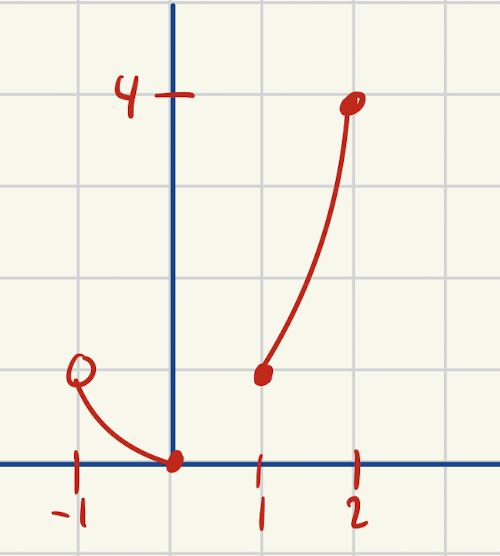
\includegraphics[width=.25\linewidth, center]{/Users/josiahvillarante/GradSchool/Grad-School-Notes/Math230A/Lecture/CH4/images/noncontinuous inverse.png}
\end{figure}

\begin{theorem} \leavevmode \\
    \label{thm4.17}
    Let $(X,d), (Y, \overset{\sim}{d})$ be metric spaces, and suppose $X$ is compact. Let $f:X \to Y$ be continuous and bijective. Then $f^{-1}:Y \to X$ is continuous.
\end{theorem}

\begin{proof}
    It is enough to show tha for every open set $B \subseteq X, (f^{-1})^{-1}(B)$ is open in $Y$. That is, suppose $B$ is open in $X$ and show $f(B)$ is open in $Y$.
    \begin{align*}
        \text{$B$ is open in $X$} &\implies \text{$B^c$ is closed in $X$} \\
        &\implies \text{$B^c$ is compact in $X$} \\
        &\implies \text{$f(B^c)$ is compact in $Y$} \\
        &\implies \text{$f(B^c)$ is closed in $Y$} \\
        &\implies \text{$[f(B^c)]^c$ is open in $Y$} \\
        &\implies \text{$f(B)$ is open in $Y$}
    \end{align*}
    \qed
\end{proof}